\documentclass[a0paper, fleqn]{tikzposter}

\title{Certifying Graph-Manipulating C Programs}
\author{Shengyi Wang$^{\dagger}$ \hspace{2ex} Qinxiang Cao$^{\ddagger}$ \hspace{2ex} \underline{Anshuman Mohan}$^{\dagger}$ \hspace{2ex} Aquinas Hobor$^{\dagger}$}
\institute{National University of Singapore$^{\dagger}$ \hspace{3ex} Shanghai Jiao Tong University$^{\ddagger}$}
\usetheme{Simple}
\usepackage{fontspec}
\defaultfontfeatures{Mapping=tex-text,Scale=MatchLowercase}
% \setmainfont{Minion Pro}
% \setsansfont{Myriad Pro}
% \setmonofont{Source Code Pro}

\colorlet{red}{red!60!black}
\colorlet{titlebgcolor}{red}
\colorlet{blocktitlefgcolor}{red}
\colorlet{maincolor}{titlebgcolor}
\colorlet{accentcolor}{titlebgcolor!40!white}
\usepackage{amsmath, amssymb, mathabx}
\usepackage{mathpartir}        % for inferrule
\usepackage{listings}
\usepackage{mathtools}         % for mathrlap
\usepackage{caption}
\usepackage{multicol}          % for multi-column listings  
\usepackage{stmaryrd}          % for the lightning symbol
\usepackage{fancyvrb}


\makeatletter
\newlength{\@mli}
\newcommand\hide[1]{}
\newcommand{\mli}[1]{%
  \settowidth{\@mli}{\lstinline/#1/}
  \hspace{-.5ex}\begin{minipage}[t]{\@mli}\lstinline/#1/\end{minipage}}
\makeatother
\newcommand{\li}[1]{\ifmmode\mbox{\mli{#1}}\else\mbox{\lstinline/#1/}\fi}
\newcommand{\infrulestyle}[1]{\textsc{#1}}
% \newcommand{\infrule}[4]{\inferrule*[lab=\infrulestyle{#1},right=$\mathrlap{#4}$]{#2}{#3}}

\newcommand{\hl}[1]{\colorbox{lightgray}{#1}}
\newcommand{\tx}[1]{\text{#1}}
\newcommand{\p}[1]{\ensuremath{\mathsf{#1}}} % predicate font
\newcommand{\m}[1]{\ensuremath{\mathit{#1}}} % math font
\newcommand{\braces}[1]{\left\{\!\!\!\begin{array}{l@{}} #1 \end{array}\right\}}
\let\ramify\lightning

\lstset{%
  language=C,
  sensitive=true,
  mathescape=true,
  showlines=true,
  basicstyle=\normalfont\tt,
  keywordstyle=\color{blocktitlebgcolor},
  numbers=left,
  numberstyle=\small,
  numbersep=5pt,
  boxpos=t,
}


\usepackage{semantic}
\newcommand{\scon}{\mathbin{\star}}

\newcommand{\ocon}{%
  \mathbin{\mbox{$\mathrlap{\cup}\hspace*{.15em}
      \raisebox{.01em}[0ex][0ex]{$\scon$}$\hspace*{.07em}}}}
\newcommand{\wand}{%
 \mathrel{\mbox{$\hspace*{-0.03em}\mathord{-}\hspace*{-0.4em}
  \mathord{-}\hspace*{-0.13em}
     \mathord{\scon}$\hspace*{-0.005em}}}}
\newcommand{\septraction}{%
  \mathrel{\mbox{$\hspace*{-0.03em}\mathord{-}\hspace*{-0.66em}
  \mathord{-}\hspace*{-0.155em}\mathord{\ocircle\hspace*{-.66em}\scon}$\hspace*{0.05em}}}}
\newcommand{\magicwand}{\wand}
\newcommand{\defeq}{\mathbin{\stackrel{\Delta}{=}}}
\newcommand{\MV}{\ensuremath{\mathsf{ModVar}}}
\newcommand{\FV}{\ensuremath{\mathsf{FreeVar}}}
\newcommand{\bigocon}{
  \raisebox{-0.3ex}{\resizebox{0.75em}{!}{$\scon$}} \hspace{-4.3ex} \bigcup}
\newcommand{\medocon}{
  \raisebox{-0.3ex}{\resizebox{0.63em}{!}{$\scon$}} \hspace{-2.05ex} \bigcup}
  \newcommand{\reachable}[5]{\ensuremath{{\m{#1}\; \stackrel{#2}{\leadsto}^{#3}_{#4} \m{#5}}}}


%\input mathlig
\mathlig{--*}{\mathrel{\magicwand}}
\mathlig{--o}{\mathrel{\septraction}}
\mathlig{|->}{\mathrel{\mapsto}} % tight points-to
\mathlig{<=>}{\mathrel{\Leftrightarrow}} % equivalence of expressions
\mathlig{==>}{\mathrel{\Rightarrow}} % meta implication
\mathlig{-|-}{\mathrel{\mathrlap{\dashv} \hspace{5pt} \vdash}} % entails

\mathlig{/|}{\mathbin{\wedge}} % additive conjunction
\mathlig{|/}{\mathbin{\vee}} % additive disjunction
\mathlig{|-}{\mathrel{\vdashtwo}} % entails
\mathlig{|=}{\vDash} % models

\mathlig{**}{\mathbin{\ocon}}
\mathlig{*}{\mathbin{\scon}}
\mathlig{//}{\color{black}{//}} % listings comments


\usepackage{tikz}
\usepackage{xcolor}
\usetikzlibrary{shadows}
\usetikzlibrary{arrows.meta, positioning, decorations.pathmorphing, fit, matrix}
\colorlet{backgroundcolor}{white}
% \titlebgcolor{\color{red}}
% \subsectionfont{\color{red}}
% \sectionfont{\color{red}}

\begin{document}
\maketitle

\node[anchor=north east,xshift=-3cm] at (TP@title.east) {
\includegraphics[scale=0.18]{badge1}};
\node[anchor=north east,yshift=5.5cm,xshift=-3cm] at (TP@title.east) {\vspace{5cm}
\includegraphics[scale=0.18]{badge2}};
\node[anchor=north west,xshift=1cm,yshift=3.5cm] at (TP@title.west) {

\includegraphics[scale=0.55]{splashlogo}};
% \node[anchor=north west,xshift=2.15cm,yshift=-3.2cm] at (TP@title.west) {OOPSLA Track};


% \begin{tikzpicture}
     % \node [anchor=north east, inner sep=3cm]  at (current page.north east)
     % {\includegraphics[scale=0.3]{badges}};
  % \end{tikzpicture}
\begin{columns}
  \column{0.5}
  \block{Overview}{%
We present a formalization of graph theory in Coq and 
a library of techniques that together mechanically 
verify \textbf{real C programs} that
manipulate \textbf{heap-represented graphs}. 

\vspace{0.5em}

\textbf{Challenge:} These structures exhibit 
\textbf{deep intrinsic sharing} and have thus historically evaded 
analysis using traditional separation logic: the \infrulestyle{frame} rule fails.

\vspace{0.5em}

\textbf{Solution:} First, we create a modular setup for reasoning about 
abstract mathematical graphs. 
Second, we add a new \infrulestyle{localize} rule to separation logic, thus
supporting existential quantifiers in postconditions and smoothly handling
modified program variables.


Our techniques are:
\begin{itemize}
\item \textbf{General and Lightweight:} We integrate our work with the CompCert and 
Verified Software Toolchain projects with minimal reengineering 
on their side. 
\item \textbf{Powerful:} We certify six graph-manipulating C programs. 
Our flagship example is a 400-line generational garbage collector.
Our proofs are entirely machine-checked in Coq.
\end{itemize}
% Paper: \emph{PACMPL \textbf{3}, OOPSLA '19, Art 171.} \includegraphics[scale=0.25]{doi}
}
% Find the full paper at 
\includegraphics[scale=0.4]{splashlogo} OOPSLA.
% \includegraphics[scale=0.3]{badges}



  \block{Workflow and Key Components}{A sketch of how we verify C programs. Note where we 
integrate with other projects.

\vspace{0.5em}

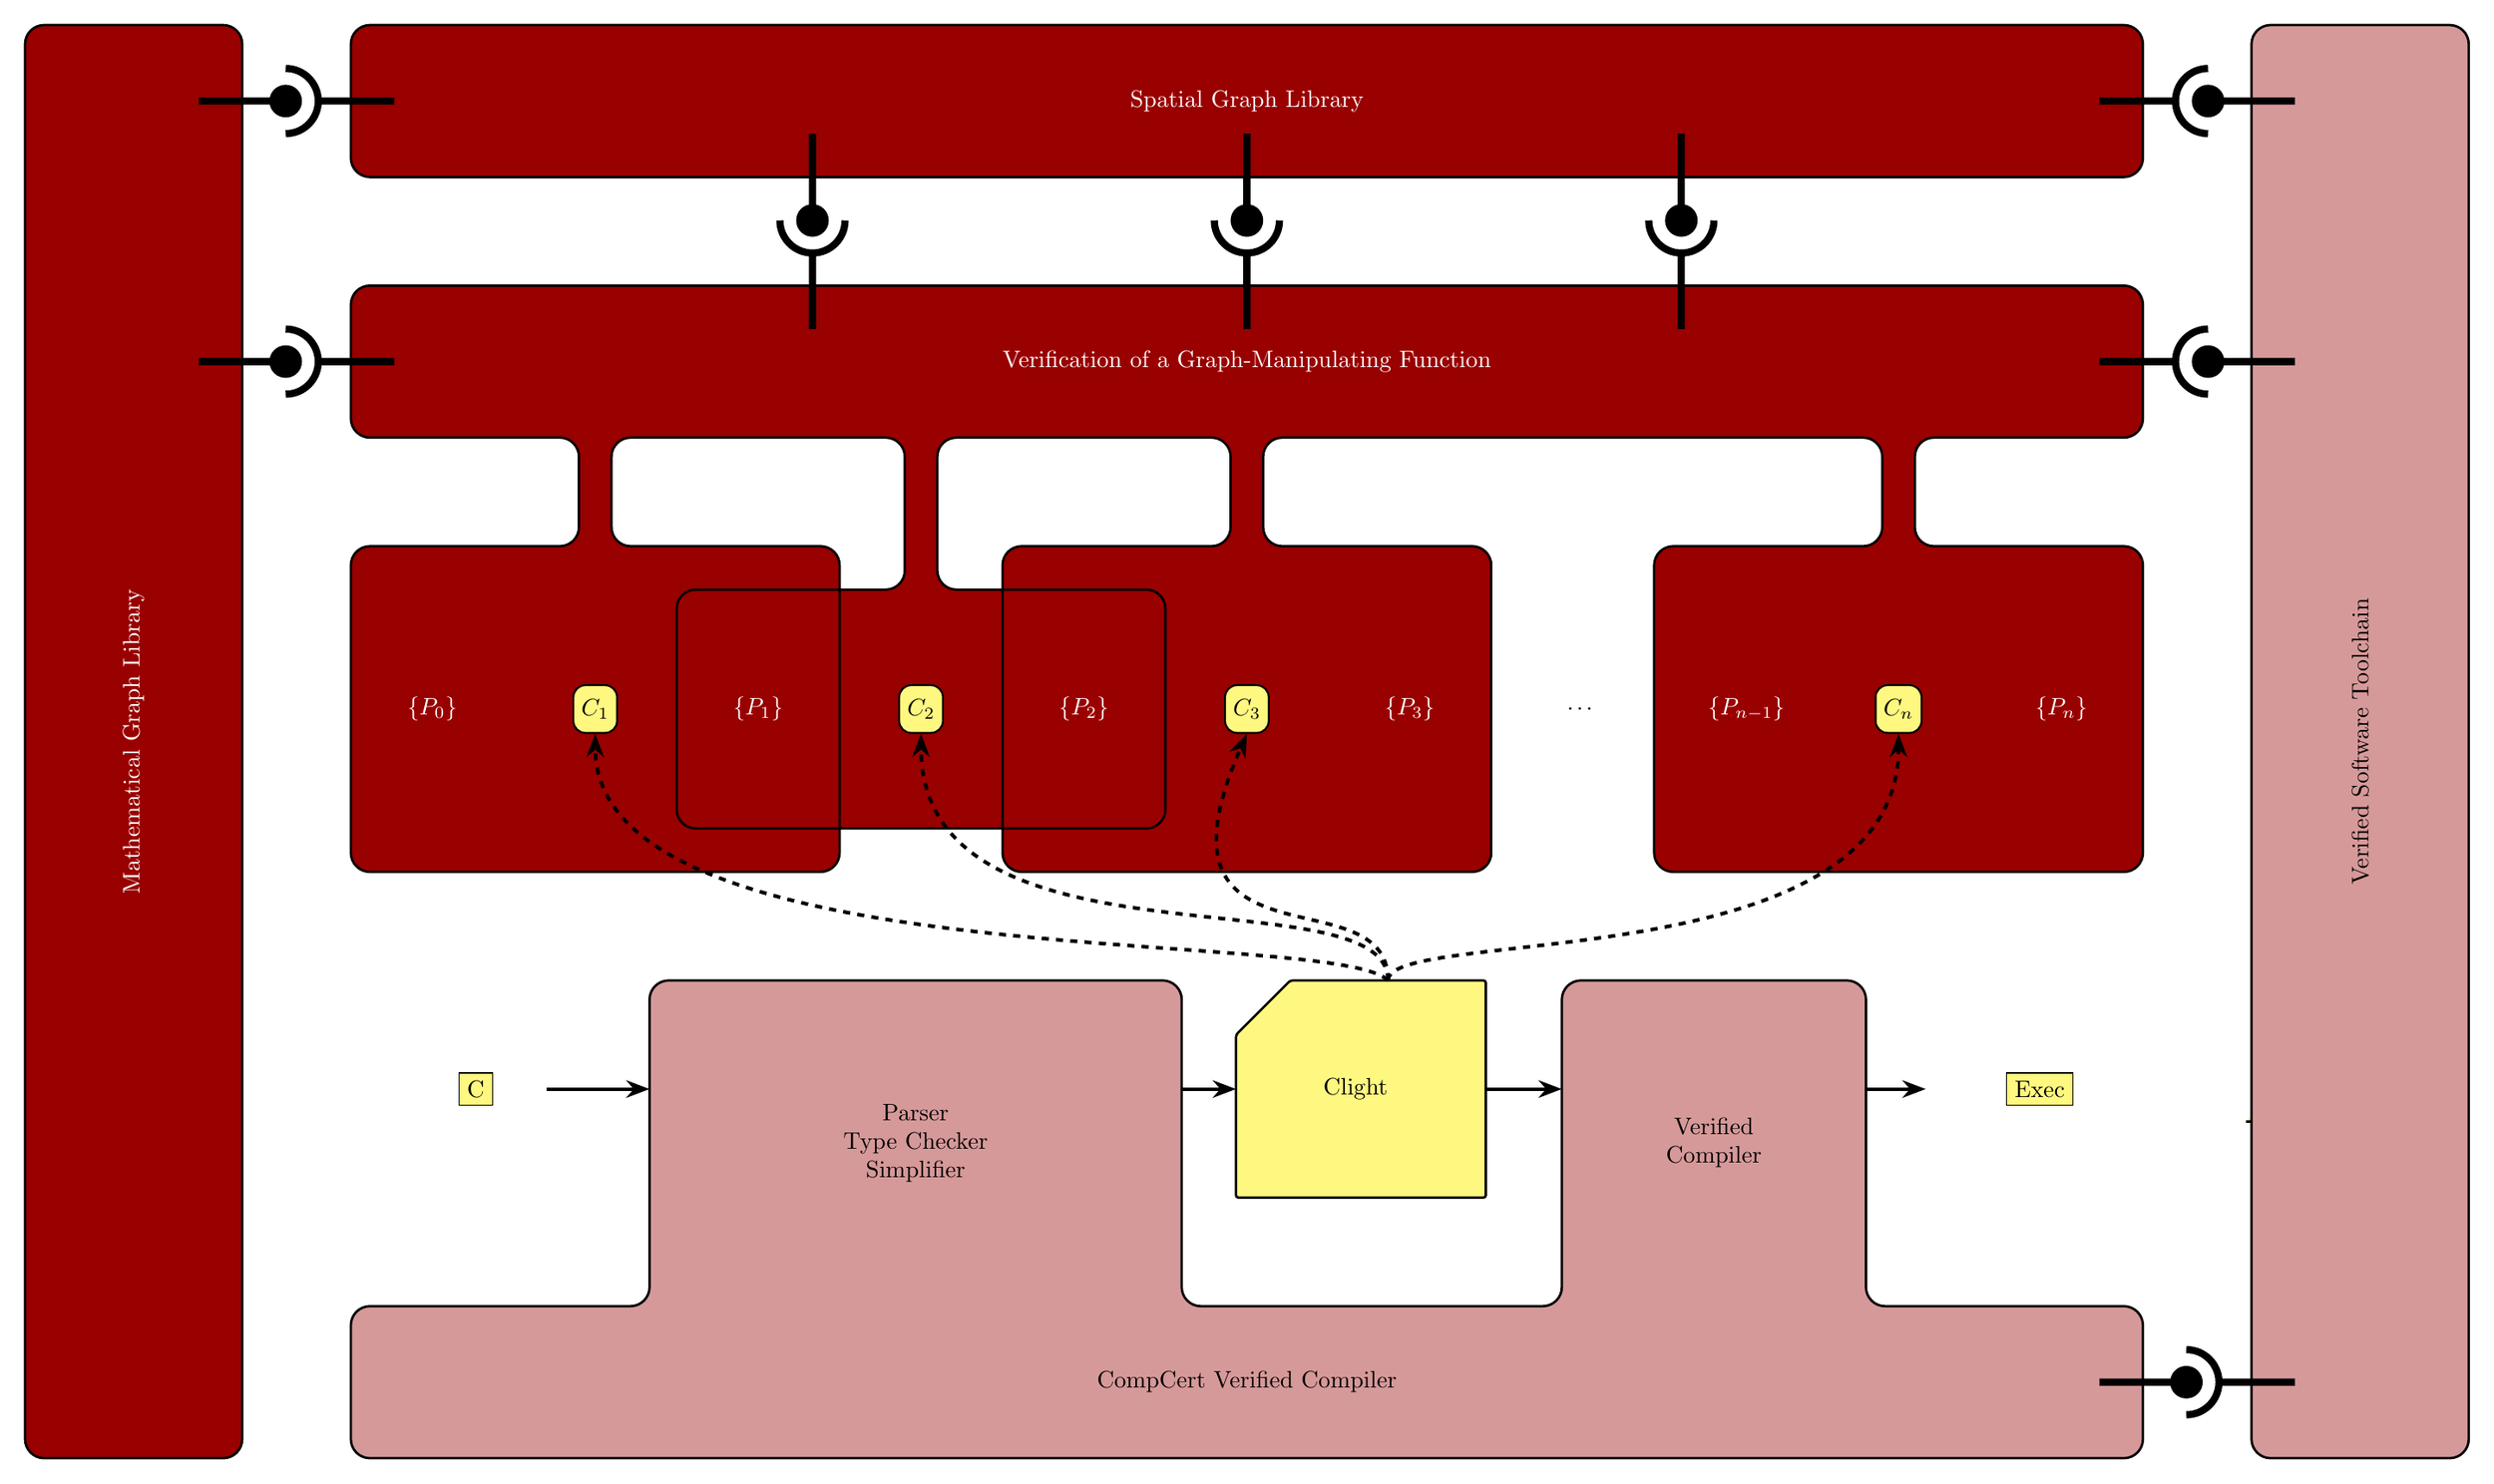
\begin{tikzpicture}[on grid, cmd/.style={rectangle, thick, fill=yellow!50!white, minimum width=2em, minimum height=1em, draw=black, rounded corners=5pt},
  ourlib/.style={rounded corners=8pt, line width=1pt},
  test/.style={rounded corners=8pt, draw=red},
  file/.style={rounded corners=1pt, line width=1pt, fill=yellow!50!white},
  ->/.style={-Stealth, line width=1.5pt}, rotate=90,transform shape, x=1.6cm, y=1.6cm]
  %% \draw [test] (-1.5, -0.5) rectangle (1.5, 2.5);
  %% \draw [test] (-1.5, 3.5) rectangle (1.5, 6.5);
  %% \draw [test] (-1.1, 5.5) rectangle (1.1, 8.5);
  %% \draw [test] (-1.5, 7.5) rectangle (1.5, 10.5);
  \draw [ourlib, fill=maincolor] (-1.5, -0.75) -- ++(3, 0) -- ++(0, 2.1) -- ++(1, 0) -- ++(0, -2.1) -- ++(1.4, 0) -- ++(0, 16.5) -- ++(-1.4, 0) --
  ++(0, -2.1) -- ++(-1, 0) -- ++(0, 2.1) -- ++(-3, 0) -- ++(0, -4.5) -- ++(3, 0) -- ++(0, 2.1) -- ++(1, 0) -- ++(0, -2.7) -- ++(-1.4, 0) -- ++(0, 2.1) --
  ++(-2.2, 0) -- ++(0, -4.5) -- ++(2.2, 0) -- ++(0, 2.1) -- ++(1.4, 0) -- ++(0, -2.7) -- ++(-1, 0) -- ++(0, 2.1) -- ++(-3, 0) -- ++(0, -4.5) -- ++(3, 0)
  -- ++(0, 2.1) -- ++(1, 0) -- ++(0, -5.7) -- ++(-1, 0) -- ++(0, 2.1) -- ++(-3, 0) -- cycle;
  \node (Pn) at (0, 0) {\rotatebox{-90}{\color{white}$\{P_n\}$}};
  \node (Pn1) [above=2.9 of Pn]  {\rotatebox{-90}{\color{white}$\{P_{n-1}\}$}};
  \node (etc) [above=1.6 of Pn1] {\vdots};
  \node (P3) [above=1.5 of etc]  {\rotatebox{-90}{\color{white}$\{P_3\}$}};
  \node (P2) [above=3 of P3]  {\rotatebox{-90}{\color{white}$\{P_2\}$}};
  \node (P1) [above=3 of P2]  {\rotatebox{-90}{\color{white}$\{P_1\}$}};
  \node (P0) [above=3 of P1]  {\rotatebox{-90}{\color{white}$\{P_0\}$}};
  \node (Cn) [above=1.5 of Pn] [cmd] {\rotatebox{-90}{$C_n$}};
  \node (C3) [above=1.5 of P3] [cmd] {\rotatebox{-90}{$C_3$}};
  \node (C2) [above=3 of C3] [cmd] {\rotatebox{-90}{$C_2$}};
  \node (C1) [above=3 of C2] [cmd] {\rotatebox{-90}{$C_1$}};

  % If I uncomment this line I get the "file", but I also get a yellow triangle below the figure.
  % I have tried various tricks to get it to go away but I can't seem to figure it out.
  % \draw [file] (-4.5, 13.95) -- ++(2, 0) -- ++ (0, 1.5) -- +(-0.5, 0.5) -- +(-2, 0.5) -- cycle ++(2, 2.3) -- ++(-0.5, 0) -- ++(0, 0.5);

  \draw [file] (-4.5, 05.30) -- ++(2, 0) -- ++ (0, 1.8) -- +(-0.5, 0.5) -- +(-2, 0.5) -- cycle ++(2, 2.3) -- ++(-0.5, 0) -- ++(0, 0.5);
  
  % \draw [file] (-4.5, -0.75) -- ++(2, 0) -- ++ (0, 1.5) -- +(-0.5, 0.5) -- +(-2, 0.5) -- cycle ++(2, 2.3) -- ++(-0.5, 0) -- ++(0, 0.5);
  
  \node[draw, fill=yellow!50!white] at (-3.5, 14.6) {\rotatebox{-90}{C}};
  \node at (-3.5, 6.5) {\rotatebox{-90}{Clight}};
  \node[draw, fill=yellow!50!white] at (-3.5, 0.2) {\rotatebox{-90}{Exec}};
  \draw [->, dashed] (-2.5, 6.2) .. controls ++(0.5, 0.5) and (-2.5, 13.5) .. (C1.west);
  \draw [->, dashed] (-2.5, 6.2) .. controls ++(1, 0) and (-2.5, 10.5) .. (C2.west);
  \draw [->, dashed] (-2.5, 6.2) .. controls ++(1, 0) and (-2.5, 8.5) .. (C3.west);
  \draw [->, dashed] (-2.5, 6.2) .. controls ++(0.5, 0) and (-2.5, 1.5) .. (Cn.west);
  \draw [->] (-3.5, 13.95) -- (-3.5, 13.0);
  \draw [->] (-3.5, 12) -- (-3.5, 7.6);
  \draw [->] (-3.5, 5.3) -- (-3.5, 4.6);
  \draw [->] (-3.5, 4.5) -- (-3.5, 1.25);
  %% \draw [test] (-6.9, -0.75) rectangle (-5.5, 15.75);
  %% \draw [test] (-4.2, 9.9) rectangle (-2.8, 11.95);
  %% \draw [test] (-4.2, 3.05) rectangle (-2.8, 5.1);
  \draw [ourlib, fill=accentcolor] (-6.9, -0.75) -- (-5.5, -0.75) -- (-5.5, 1.8) -- (-2.5, 1.8) -- (-2.5, 4.6) -- (-5.5, 4.6) -- (-5.5, 8.1) --
  (-2.5, 8.1) -- (-2.5, 13.0) -- (-5.5, 13) -- (-5.5, 15.75) -- (-6.9, 15.75) -- cycle;
  \node at (-4, 10.55) {\rotatebox{-90}{\begin{tabular}{c} Parser\\ Type Checker \\ Simplifier \end{tabular}}};
  \node at (-4, 3.2) {\rotatebox{-90}{\begin{tabular}{c} Verified \\ Compiler \end{tabular}}};
  \node at (-6.2, 7.5) {\rotatebox{-90}{CompCert Verified Compiler}};
  \draw [ourlib, fill=accentcolor] (-6.9, -3.75) rectangle (6.3, -1.75);
  \node at (-0.3, -2.75) {Verified Software Toolchain};
  \draw [ourlib, fill=maincolor] (-6.9, 16.75) rectangle (6.3, 18.75);
  \node at (-0.3, 17.75) {\color{white}Mathematical Graph Library};
  \node at (3.2, 7.5) {\rotatebox{-90}{\color{white}Verification of a Graph-Manipulating Function}};
  \draw [ourlib, fill=maincolor] (4.9, -0.75) rectangle (6.3, 15.75);
  \node at (5.6, 7.5) {\rotatebox{-90}{\color{white}Spatial Graph Library}};

  %% down interface
  \draw [line width=3pt] (5.6, -0.35) -- +(0, -0.7) +(0, -1.05) -- +(0, -1.8) +(0.3, -1) arc [start angle=0, end angle=180, radius=0.3];
  \fill (5.6, -1.35) circle [radius=0.15];
  \draw [line width=3pt] (3.2, -0.35) -- +(0, -0.7) +(0, -1.05) -- +(0, -1.8) +(0.3, -1) arc [start angle=0, end angle=180, radius=0.3];
  \fill (3.2, -1.35) circle [radius=0.15];

  %% up interface
  \draw [line width=3pt] (-6.2, -2.15) -- +(0, 0.7) +(0, 1.05) -- +(0, 1.8) +(0.3, 1) arc [start angle=0, end angle=-180, radius=0.3];
  \fill (-6.2, -1.15) circle [radius=0.15];
  \draw [line width=3pt] (3.2, 15.35) -- +(0, 0.7) +(0, 1.05) -- +(0, 1.8) +(0.3, 1) arc [start angle=0, end angle=-180, radius=0.3];
  \fill (3.2, 16.35) circle [radius=0.15];
  \draw [line width=3pt] (5.6, 15.35) -- +(0, 0.7) +(0, 1.05) -- +(0, 1.8) +(0.3, 1) arc [start angle=0, end angle=-180, radius=0.3];
  \fill (5.6, 16.35) circle [radius=0.15];

  %% right interface
  \draw [line width=3pt] (3.5, 7.5) -- +(0.7, 0) +(1.05, 0) -- +(1.8, 0) +(1, 0.3) arc [start angle=90, end angle=270, radius=0.3];
  \fill (4.5, 7.5) circle [radius=0.15];
  \draw [line width=3pt] (3.5, 11.5) -- +(0.7, 0) +(1.05, 0) -- +(1.8, 0) +(1, 0.3) arc [start angle=90, end angle=270, radius=0.3];
  \fill (4.5, 11.5) circle [radius=0.15];  
  \draw [line width=3pt] (3.5, 3.5) -- +(0.7, 0) +(1.05, 0) -- +(1.8, 0) +(1, 0.3) arc [start angle=90, end angle=270, radius=0.3];
  \fill (4.5, 3.5) circle [radius=0.15];
\end{tikzpicture}
}
  % \block{}{\centering\begin{tabular}{c|c|c|c|c}
Component & Files & Size (loc) & Definitions & Theorems\\\hline
Common Utilities & 10 & 3,578 & 44 & 289 \\
Math Graph Library &  20 & 10,585 & 216 & 581 \\
Spatial Graph Library &  3 & 2,328 & 59 & 110 \\
Integration into VST & 11 & 2,783 & 17 & 172 \\
\hline
Marking (graph and DAG) &  6 & 775 & 9 & 20 \\
Spanning Tree & 5 & 2,723 & 17 & 92 \\
Union-Find (heap and array) &  18 & 3,193 & 107 & 135 \\
Garbage Collector & 16 & 13,858 & 235 & 712 \\
% \hline & & & &  \\
% [-2.2em] \\
% \hline & & & & \\
\hline
Total Development & 89 & 39,823 & 704 & 2,111 \\
\end{tabular}
\hide{
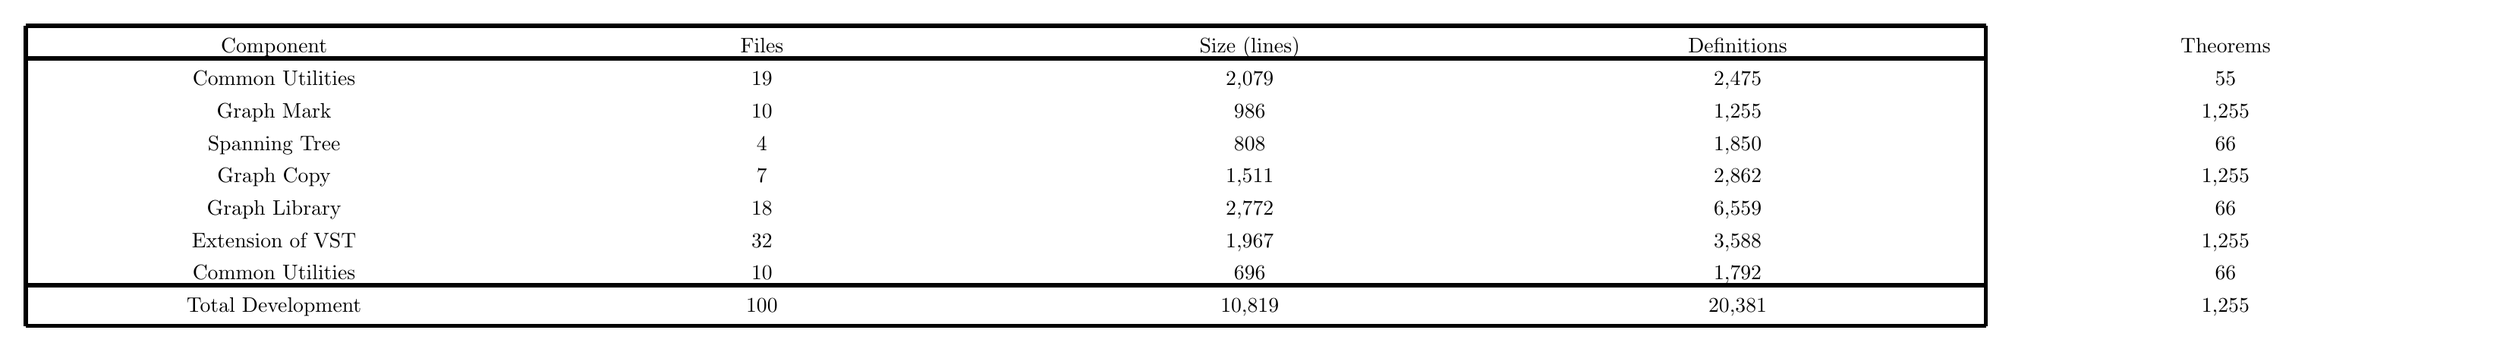
\begin{tikzpicture}[line width = 2pt]
  \matrix(stat)[
    matrix of nodes,
    ampersand replacement=\&,
    nodes={rectangle, align=center,text width=8cm},
    row sep=-\pgflinewidth,
    column sep=-\pgflinewidth,
    text depth=0.5ex,
    text height=2ex
  ]{
    |[fill=backgroundcolor]| Component \& |[fill=backgroundcolor]| Files \& |[fill=backgroundcolor]| Size (lines) \& |[fill=backgroundcolor]| Definitions \& |[fill=backgroundcolor]| Theorems \\
    Common Utilities  \& 19 \& 2,079 \& 2,475 \& 55 \\ 
    |[fill=backgroundcolor]| Graph Mark \& |[fill=backgroundcolor]| 10 \& |[fill=backgroundcolor]| 986 \& |[fill=backgroundcolor]| 1,255 \& |[fill=backgroundcolor]| 1,255 \\
    Spanning Tree  \& 4 \& 808 \& 1,850 \& 66 \\
    |[fill=backgroundcolor]| Graph Copy \& |[fill=backgroundcolor]| 7 \& |[fill=backgroundcolor]| 1,511 \& |[fill=backgroundcolor]| 2,862 \& |[fill=backgroundcolor]| 1,255\\
    Graph Library \& 18 \& 2,772 \& 6,559 \& 66\\
    |[fill=backgroundcolor]| Extension of VST  \& |[fill=backgroundcolor]| 32 \& |[fill=backgroundcolor]| 1,967 \& |[fill=backgroundcolor]| 3,588 \& |[fill=backgroundcolor]| 1,255\\
    Common Utilities \& 10 \& 696 \& 1,792 \& 66\\
    |[fill=backgroundcolor]| Total Development \& |[fill=backgroundcolor]| 100 \& |[fill=backgroundcolor]| 10,819 \& |[fill=backgroundcolor]| 20,381 \& |[fill=backgroundcolor]| 1,255\\
  };
  \draw(stat-1-1.north west)--(stat-1-4.north east);
  \draw(stat-2-1.north west)--(stat-2-4.north east);
  \draw(stat-9-1.north west)--(stat-9-4.north east);
  \draw(stat-9-1.south west)--(stat-9-4.south east);
  \draw(stat-1-1.north west)--(stat-9-1.south west);
  \draw(stat-1-4.north east)--(stat-9-4.south east);
\end{tikzpicture}
}}

  % \block{}{\centering\input{poster_pregraph.tex}}
  \block{}{
The structure of our Mathematical Graph Library.
The soundness condition is entirely customizable.
Lemmas and properties can be composed, and are automatically inherited.

\vspace{0.5em}
\hspace{-2.75ex}\centering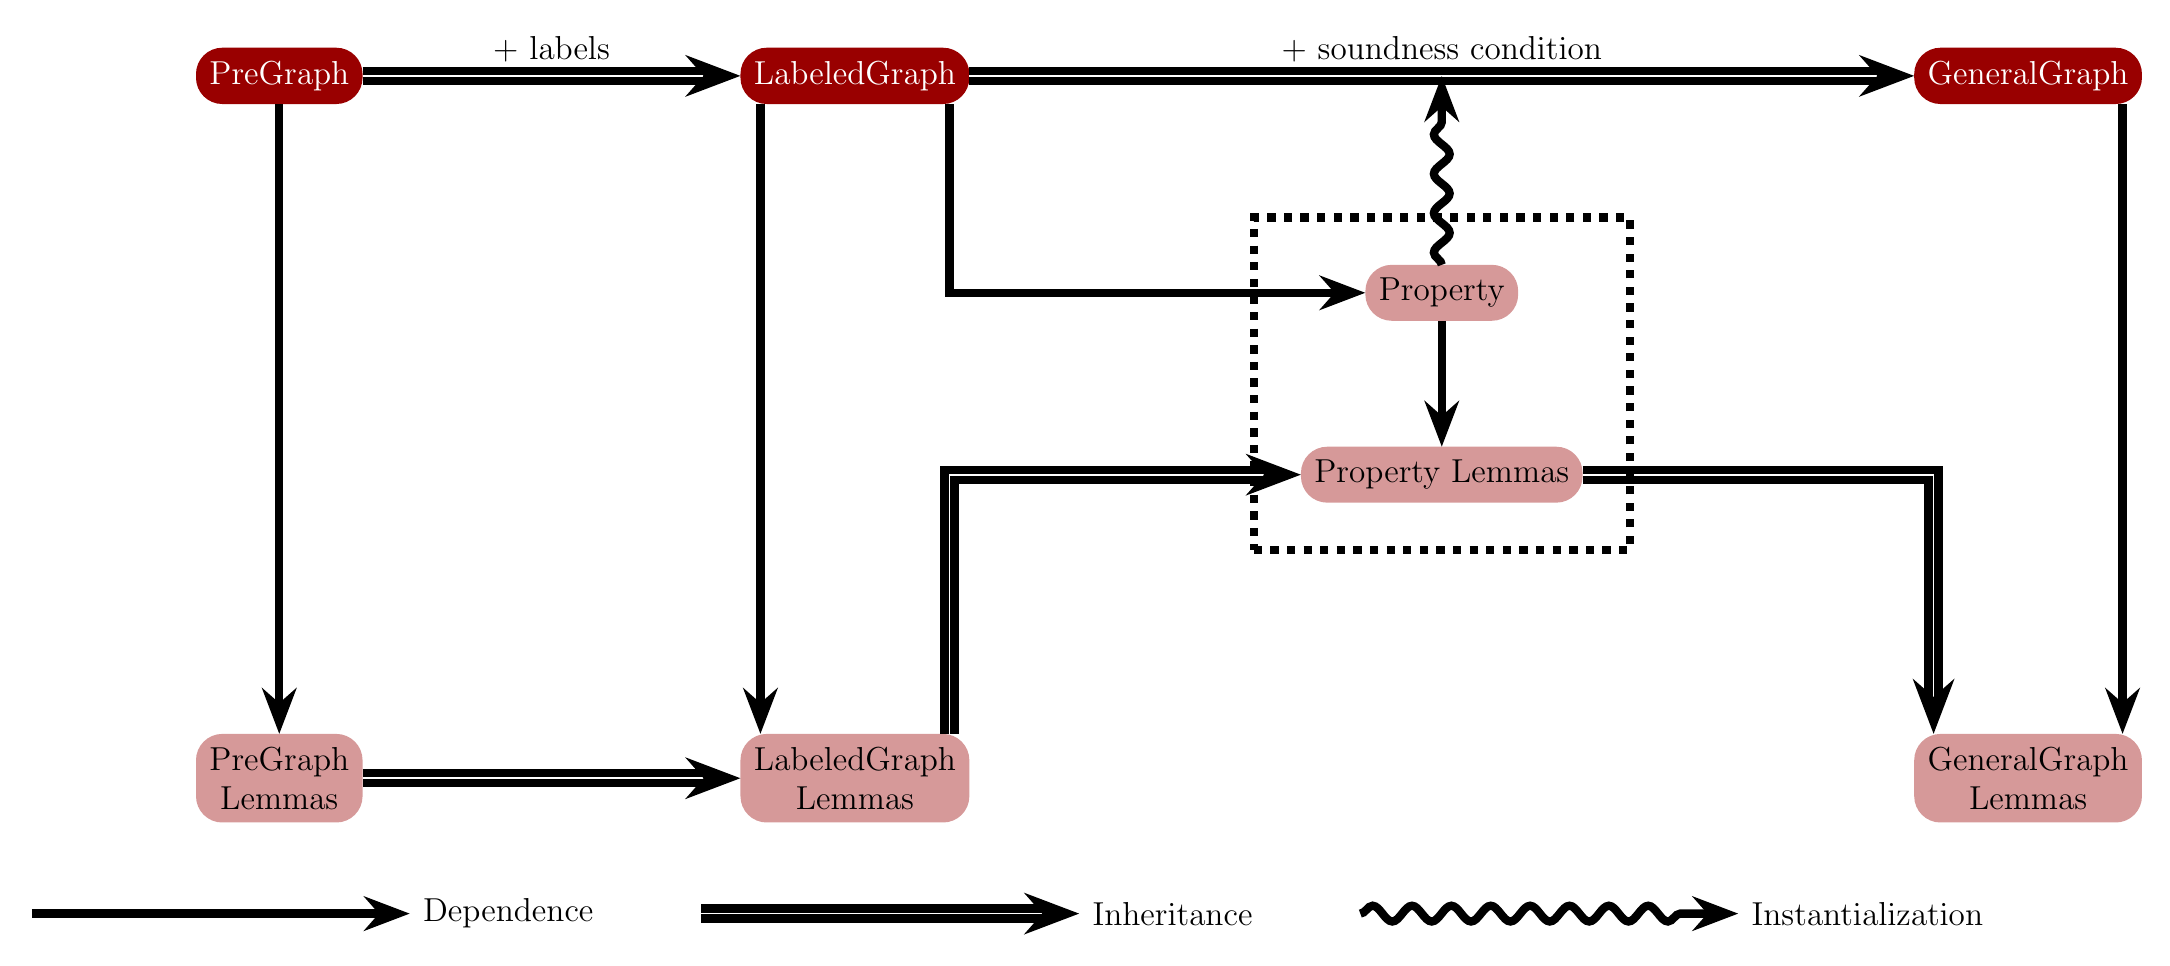
\begin{tikzpicture}
  [every shadow/.style={opacity=0.0, shadow xshift=8pt, shadow yshift=-8pt},
    ->/.style={line width=3pt, arrows={-Stealth}},
    -->/.style={line width=3pt, arrows={-Stealth}, decorate, decoration={snake, amplitude=1mm,segment length=5mm,post length=5mm}},
    realG/.style={shape=rectangle, rounded corners=8pt, text=white, draw=maincolor, fill=maincolor, drop shadow},
    propG/.style={shape=rectangle, rounded corners=8pt, text=black, draw=accentcolor, fill=accentcolor, drop shadow},
    x=6cm, y=4cm, line width=3pt, font=\large]
\node[realG] (PG) at (0, 0) { PreGraph};
\node[realG] (LG) [right=0.8 of PG] { LabeledGraph};
\node[realG] (GG) [right=2 of LG] { GeneralGraph};
\draw [double, ->] (PG) -- (LG) node [pos=0.5, above] { $+$ labels} ;
\draw [double, ->] (LG) -- (GG) node (SC) [pos=0.5, above, align=center]
{ $+$ soundness condition};
\node[propG] (Prop) [below=0.6 of SC] { Property};
\node[propG] (PropL) [below=0.4 of Prop] { Property Lemmas};
\node[propG] (PGL) [below=2 of PG, align=center] { PreGraph \\ Lemmas};
\node[propG] (LGL) [below=2 of LG, align=center] { LabeledGraph \\ Lemmas};
\node[propG] (GGL) [below=2 of GG, align=center] { GeneralGraph \\ Lemmas};
\draw [double, ->] (PGL) to (LGL);
%% \draw [double, ->] (LGL) to (GGL);
\draw [->] (PG) to (PGL);
\draw [->] (Prop) to (PropL);
\draw [-->] (Prop) to (SC);
\coordinate [left=0.2 of LG.south] (LGs1);
\coordinate [left=0.2 of LGL.north] (LGLn1);
\draw [->] (LGs1) to (LGLn1);
\coordinate [right=0.2 of LG.south] (LGs2);
\coordinate [right=0.2 of LGL.north] (LGLn2);
\draw [->] (LGs2) |- (Prop);
\draw [double, ->] (LGLn2) |- (PropL);
\coordinate [right=0.2 of GG.south] (GGs);
\coordinate [left=0.2 of GGL.north] (GGLn1);
\coordinate [right=0.2 of GGL.north] (GGLn2);
\draw [double, ->] (PropL) -| (GGLn1);
\draw [->] (GGs) to (GGLn2);
\node [draw, rectangle, dashed, inner sep=0.6cm, fit=(Prop) (PropL)] {};
\node (legend1) [below right=0.2 and 0.1 of PGL] { Dependence};
\coordinate[left=0.8 of legend1]  (l1);
\draw [->] (l1) to (legend1);
\node (legend2) [right=1 of legend1] { Inheritance};
\coordinate[left=0.8 of legend2]  (l2);
\draw [double, ->] (l2) to (legend2);
\node (legend3) [right=1 of legend2] { Instantialization};
\coordinate[left=0.8 of legend3]  (l3);
\draw [-->] (l3) to (legend3);
\end{tikzpicture}
% \captionof{figure}{Structure of the Mathematical Graph Library}}

  \block{}{
Our key addition to separation logic. The rule below is 
coderivable from the \infrulestyle{frame} rule.

  \begin{equation*}
\inferrule [localize] 
{G_1 \vdash L_1 * R  \\
\{ L_1 \} ~ c ~ \{ \exists x.~ L_2 \} \\
R \vdash \forall x.~ (L_2 \wand G_2) }
{\{ G_1 \} ~ c ~ \{ \exists x.~ G_2 \}}
\; \FV(R) \cap \MV(c) = \emptyset \qquad
% {G_1 |- L_1 * R  \\
% \{ L_1 \} ~ c ~ \{ \exists x.~ L_2 \} \\
% R |- \forall x.~ (L_2 --* G_2) }
% {\{ G_1 \} ~ c ~ \{ \exists x.~ G_2 \}} 
% {\FV(R) \cap \MV(c) = \emptyset \qquad}
\end{equation*}}

\block{}{
Some statistics relating to our development.
\vspace{0.5em}

\centering\begin{tabular}{c|c|c|c|c}
Component & Files & Size (loc) & Definitions & Theorems\\\hline
Common Utilities & 10 & 3,578 & 44 & 289 \\
Math Graph Library &  20 & 10,585 & 216 & 581 \\
Spatial Graph Library &  3 & 2,328 & 59 & 110 \\
Integration into VST & 11 & 2,783 & 17 & 172 \\
\hline
Marking (graph and DAG) &  6 & 775 & 9 & 20 \\
Spanning Tree & 5 & 2,723 & 17 & 92 \\
Union-Find (heap and array) &  18 & 3,193 & 107 & 135 \\
Garbage Collector & 16 & 13,858 & 235 & 712 \\
% \hline & & & &  \\
% [-2.2em] \\
% \hline & & & & \\
\hline
Total Development & 89 & 39,823 & 704 & 2,111 \\
\end{tabular}
\hide{
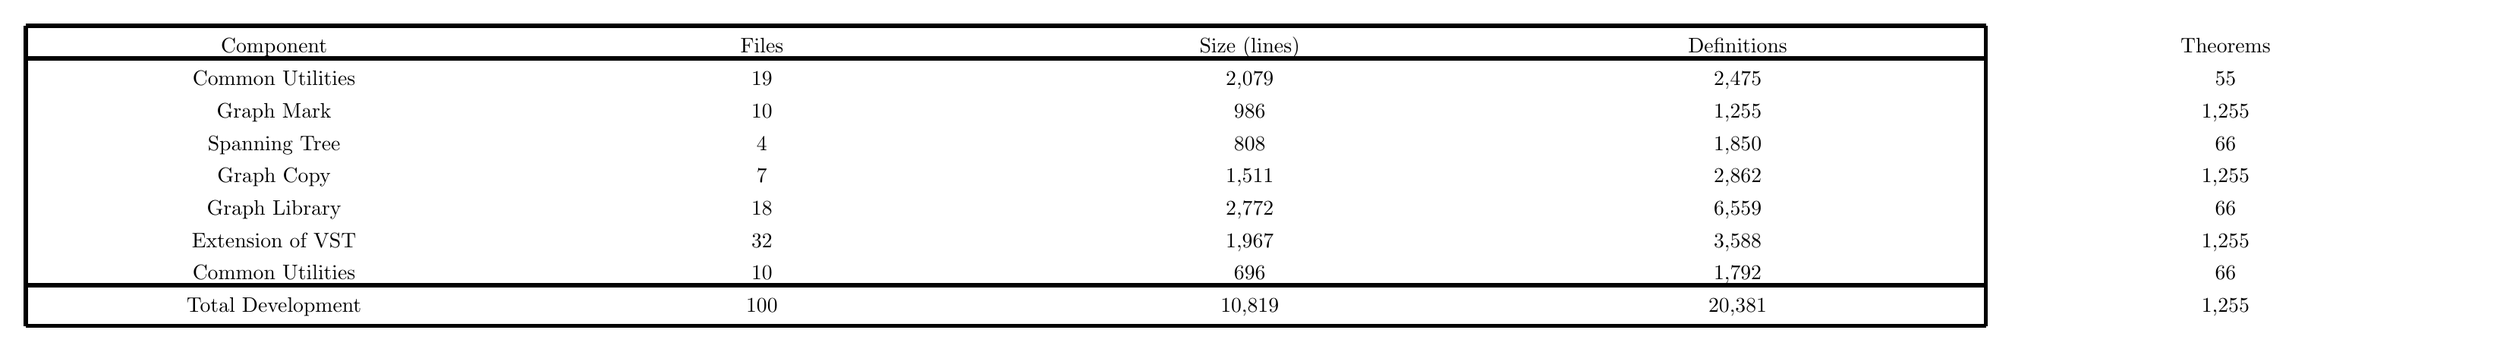
\begin{tikzpicture}[line width = 2pt]
  \matrix(stat)[
    matrix of nodes,
    ampersand replacement=\&,
    nodes={rectangle, align=center,text width=8cm},
    row sep=-\pgflinewidth,
    column sep=-\pgflinewidth,
    text depth=0.5ex,
    text height=2ex
  ]{
    |[fill=backgroundcolor]| Component \& |[fill=backgroundcolor]| Files \& |[fill=backgroundcolor]| Size (lines) \& |[fill=backgroundcolor]| Definitions \& |[fill=backgroundcolor]| Theorems \\
    Common Utilities  \& 19 \& 2,079 \& 2,475 \& 55 \\ 
    |[fill=backgroundcolor]| Graph Mark \& |[fill=backgroundcolor]| 10 \& |[fill=backgroundcolor]| 986 \& |[fill=backgroundcolor]| 1,255 \& |[fill=backgroundcolor]| 1,255 \\
    Spanning Tree  \& 4 \& 808 \& 1,850 \& 66 \\
    |[fill=backgroundcolor]| Graph Copy \& |[fill=backgroundcolor]| 7 \& |[fill=backgroundcolor]| 1,511 \& |[fill=backgroundcolor]| 2,862 \& |[fill=backgroundcolor]| 1,255\\
    Graph Library \& 18 \& 2,772 \& 6,559 \& 66\\
    |[fill=backgroundcolor]| Extension of VST  \& |[fill=backgroundcolor]| 32 \& |[fill=backgroundcolor]| 1,967 \& |[fill=backgroundcolor]| 3,588 \& |[fill=backgroundcolor]| 1,255\\
    Common Utilities \& 10 \& 696 \& 1,792 \& 66\\
    |[fill=backgroundcolor]| Total Development \& |[fill=backgroundcolor]| 100 \& |[fill=backgroundcolor]| 10,819 \& |[fill=backgroundcolor]| 20,381 \& |[fill=backgroundcolor]| 1,255\\
  };
  \draw(stat-1-1.north west)--(stat-1-4.north east);
  \draw(stat-2-1.north west)--(stat-2-4.north east);
  \draw(stat-9-1.north west)--(stat-9-4.north east);
  \draw(stat-9-1.south west)--(stat-9-4.south east);
  \draw(stat-1-1.north west)--(stat-9-1.south west);
  \draw(stat-1-4.north east)--(stat-9-4.south east);
\end{tikzpicture}
}}


    \column{0.5}
  \block{Annotated Proof Sketch for \texttt{find}}{\colorlet{stash}{red}
\colorlet{red}{maincolor}

\begin{lstlisting}
  struct Node { unsigned int rank;
                struct Node * parent; }
  $//$$\left\{\p{uf\_graph}(\gamma) /| \tx{x}\in\m{V}(\gamma)\right\}$
  struct Node* find(struct Node* x) {
    struct Node *p;
  $//$$\left\{\begin{array}{l@{}} \p{uf\_graph}(\gamma) /| \tx{x}\in\m{V}(\gamma) /| \null \\ {\color{red}\exists\m{r},\m{pa}.~\gamma(\tx{x}) = (\m{r}, \m{pa})} /| {\color{red}\m{pa}\in\m{V}(\gamma)} \end{array} \right\}$
  $//$$\searrow \left\{\begin{array}{l@{}} {\color{red}\tx{x} \mapsto \m{r},\m{pa}} /| \tx{x}\in\m{V}(\gamma) /| \null \\ \gamma(\tx{x}) = (\m{r}, \m{pa}) /| \m{pa}\in\m{V}(\gamma) \end{array}\right\}$
  $\ramify$  p = x -> parent;
  $//$$\swarrow \left\{\begin{array}{l@{}} \tx{x}\mapsto \m{r},\m{pa} /| {\color{red}\tx{p} = \m{pa}} /| \tx{x}\in\m{V}(\gamma) /| \null \\ \gamma(\tx{x}) = (\m{r}, \m{pa}) /| \m{pa}\in\m{V}(\gamma)\end{array}\right\}$
  $//$$\left\{\begin{array}{l@{}} {\color{red}\p{uf\_graph}(\gamma)} /| \tx{p} = \m{pa} /| \tx{x}\in\m{V}(\gamma) /| \null \\ \gamma(\tx{x}) = (\m{r}, \m{pa}) /| \m{pa}\in\m{V}(\gamma)\end{array}\right\}$
    if (p != x) { 
  $//$$\left\{\begin{array}{l@{}} \p{uf\_graph}(\gamma) /| \tx{p} = \m{pa} /| {\color{red}\m{pa} \neq \tx{x}} /| \null \\ \tx{x}\in\m{V}(\gamma) /| \gamma(\tx{x}) = (\m{r}, \m{pa}) /| \m{pa}\in\m{V}(\gamma)\end{array}\right\}$
      p = find(p);
  $//$$\left\{\begin{array}{l@{}}{\color{red}\exists \gamma',\m{rt}.~\p{uf\_graph}(\gamma')} /| {\color{red}\tx{p} = \m{rt}} /| \m{pa} \neq \tx{x} /| \tx{x}\in\m{V}(\gamma) /| \null \\ {\color{red}\m{findS}(\gamma,\m{pa},\gamma')} /| {\color{red}\m{uf\_root}(\gamma',\m{pa},\m{rt})} /|  \gamma(\tx{x})=(\m{r},\m{pa})\end{array}\right\}$
  $//$$\searrow \left\{\begin{array}{l@{}}{\color{red}\tx{x} \mapsto \m{r},{pa}} /| \tx{p} = \m{rt} /| \m{pa} \neq \tx{x} /| \m{findS}(\gamma, \m{pa}, \gamma') /| \null \\ \m{uf\_root}(\gamma',\m{pa},\m{rt}) /| \tx{x}\in\m{V}(\gamma) /| \gamma(\tx{x})=(\m{r}, \m{pa})\end{array}\right\}$
  $\ramify$    x -> parent = p;
  $//$$\swarrow \left\{\begin{array}{l@{}}\tx{x} \mapsto \m{r},{\color{red}\m{rt}} /| \tx{p} = \m{rt} /| \m{pa} \neq \tx{x} /| \m{findS}(\gamma, \m{pa}, \gamma') /| \null \\ \m{uf\_root}(\gamma',\m{pa},\m{rt}) /| \tx{x}\in\m{V}(\gamma) /| \gamma(\tx{x})=(\m{r}, \m{pa})\end{array}\right\}$
  $//$$\left\{\begin{array}{l@{}} {\color{red}\exists \gamma''.~ \p{uf\_graph}(\gamma'')} /| {\color{red}\m{findS}(\gamma, \m{pa}, \gamma'')} /| \null \\ {\color{red}\m{uf\_root}(\gamma'',\tx{x},\m{rt})} /| \tx{p} = \m{rt} \end{array}\right\}$
    } return p;
  } $//$$ \left\{\begin{array}{l@{}} \exists \gamma'',\m{rt}.~\p{uf\_graph}(\gamma'') /| \m{findS}(\gamma, \tx{x}, \gamma'') /| \null \\\m{uf\_root}(\gamma'',\tx{x},\m{rt}) /| {\color{red}\tx{ret} = \m{rt}}  \end{array}\right\}$
\end{lstlisting}

%
%\begin{minipage}[c]{\textwidth} \hline \end{minipage}
%
\vspace*{-1ex}

\begin{flushleft}
% \begin{minipage}[c]{0.46\textwidth}
% \vspace*{-1ex}
\begin{equation*}
\begin{array}{@{}l@{}lcl@{}}
\multicolumn{2}{r}{\p{uf\_graph}(x, \gamma)} & \defeq & \underset{\m{v} \in \m{V}(\gamma)}{\bigstar} \m{v}	\mapsto\gamma(\m{v}) \\
[25pt]
\m{uf\_root}(\gamma,\m{x},\m{rt})&& \defeq & \reachable{x}{\gamma}{\star}{}{rt} \; /| {\forall \m{rt'}.~\reachable{rt}{\gamma}{\star}{}{rt'} => \m{rt} = \m{rt'}}
\end{array}
\end{equation*}
% \end{minipage}
% \vline
% \begin{minipage}[c]{0.5\textwidth}
% \vspace*{1ex}
\begin{equation*}
\begin{split}
\quad \m{findS}(\gamma,\m{x},\gamma') \; \defeq \; &\big(\forall \m{v}.~ \m{v}\in\m{V}(\gamma) <=> \m{v}\in\m{V}(\gamma') \big) /| \null \\
&\big(\forall \m{v}.~\m{v}\in\m{V}(\gamma) => \gamma(\m{v}).\m{rank} = \gamma'(\m{v}).\m{rank} \big) /| \null \\
&\big(\forall \m{r},\m{r'}.~\m{uf\_root}(\gamma, \m{v}, \m{r}) => \m{uf\_root}(\gamma', \m{v}, \m{r'}) => \m{r} = \m{r'} \big) /|  \null \\
&\big(\gamma \smallsetminus \{\m{v} \in \gamma \mid \reachable{x}{\gamma}{\star}{}{v}\} \cong \gamma' \smallsetminus \{\m{v} \in \gamma \mid \reachable{x}{\gamma}{\star}{}{v}\}\big)
\end{split}
\end{equation*}
% \end{minipage}
\end{flushleft}

\colorlet{red}{stash}
}

\block{Verification of Garbage Collector}{
We verify a \textbf{generational garbage collector} for the CertiCoq Project.
It is \mbox{$\approx400$} lines long, and is based on the OCaml GC: 
\textbf{12 generations}, 
\textbf{variable-sized blocks}, and 
\textbf{runtime disambiguation} of boxed/unboxed fields.

\vspace{0.5em}
We identify two areas where ANSI C semantics are too weak to certify OCaml-style GCs:
  \begin{itemize}
  \item Double-bounded pointer comparisons:

\texttt{int Is\_from(value * from\_start, value * from\_limit, value * v) \{ }
\vspace{-0.3em}
\texttt{    return (from\_start <= v \&\& v < from\_limit); \} }

  \item A classic OCaml trick for runtime disambiguation of fields:
  
\texttt{int test\_int\_or\_ptr (value x) \{ return (int)(((intnat)x)\&1); \} }

\end{itemize}

Both tests, although undefined in C, 
are compatible with the CompCert compiler.
% via \texttt{extcall\_properties}.

\noindent Below we present a visualization of the theorems involved in the proof.

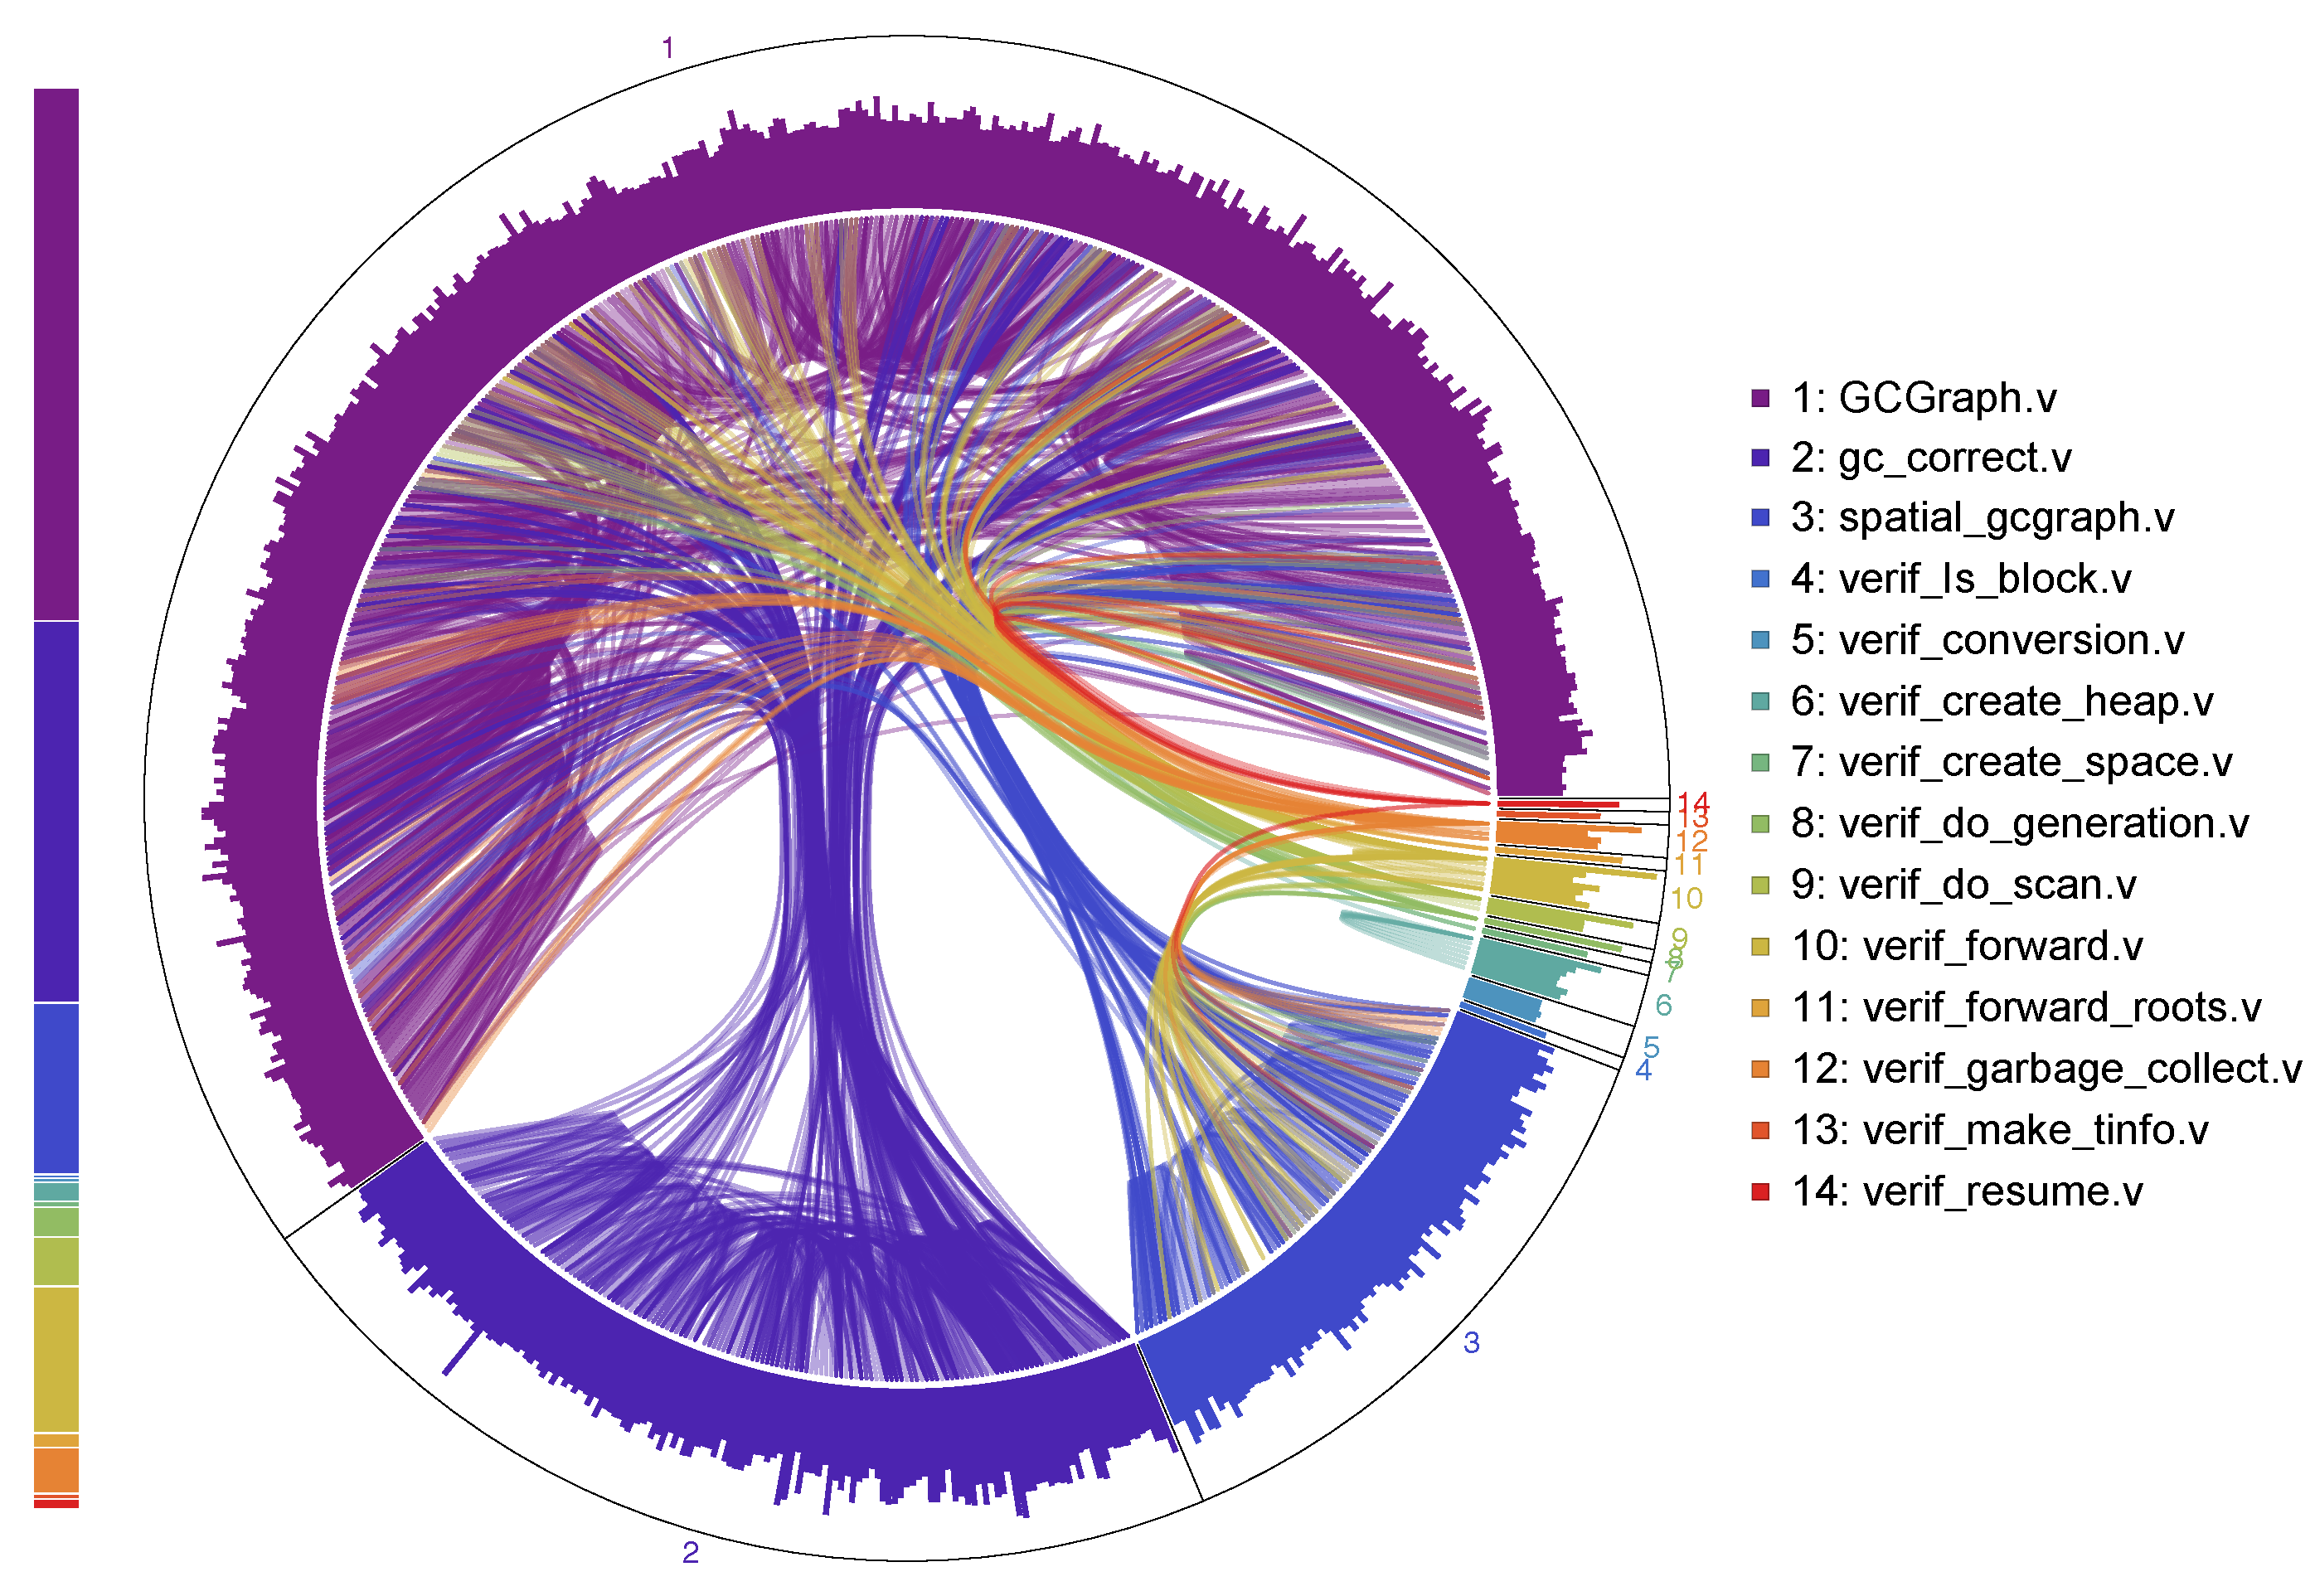
\includegraphics[width=0.4\textwidth]{certigc_theorems}

}



  %% \block{Combining plugins}{\centering\input{poster_plugin.tex}}
  
  %% \block{Statistics Related to Our Development}{ All of our
  %%   verification has been machine-checked in Coq. Although the size of
  %%   a development does not perfectly match with that development's
  %%   importance or implementation difficulty, we present it nonetheless
  %%   in the following table. We list not only the size of concrete
  %%   verification of various algorithms, but also the size of the
  %%   infrastructure of the library.
    
  %%   \vspace{0.5cm}
  %%   \centering\begin{tabular}{c|c|c|c|c}
Component & Files & Size (loc) & Definitions & Theorems\\\hline
Common Utilities & 10 & 3,578 & 44 & 289 \\
Math Graph Library &  20 & 10,585 & 216 & 581 \\
Spatial Graph Library &  3 & 2,328 & 59 & 110 \\
Integration into VST & 11 & 2,783 & 17 & 172 \\
\hline
Marking (graph and DAG) &  6 & 775 & 9 & 20 \\
Spanning Tree & 5 & 2,723 & 17 & 92 \\
Union-Find (heap and array) &  18 & 3,193 & 107 & 135 \\
Garbage Collector & 16 & 13,858 & 235 & 712 \\
% \hline & & & &  \\
% [-2.2em] \\
% \hline & & & & \\
\hline
Total Development & 89 & 39,823 & 704 & 2,111 \\
\end{tabular}
\hide{
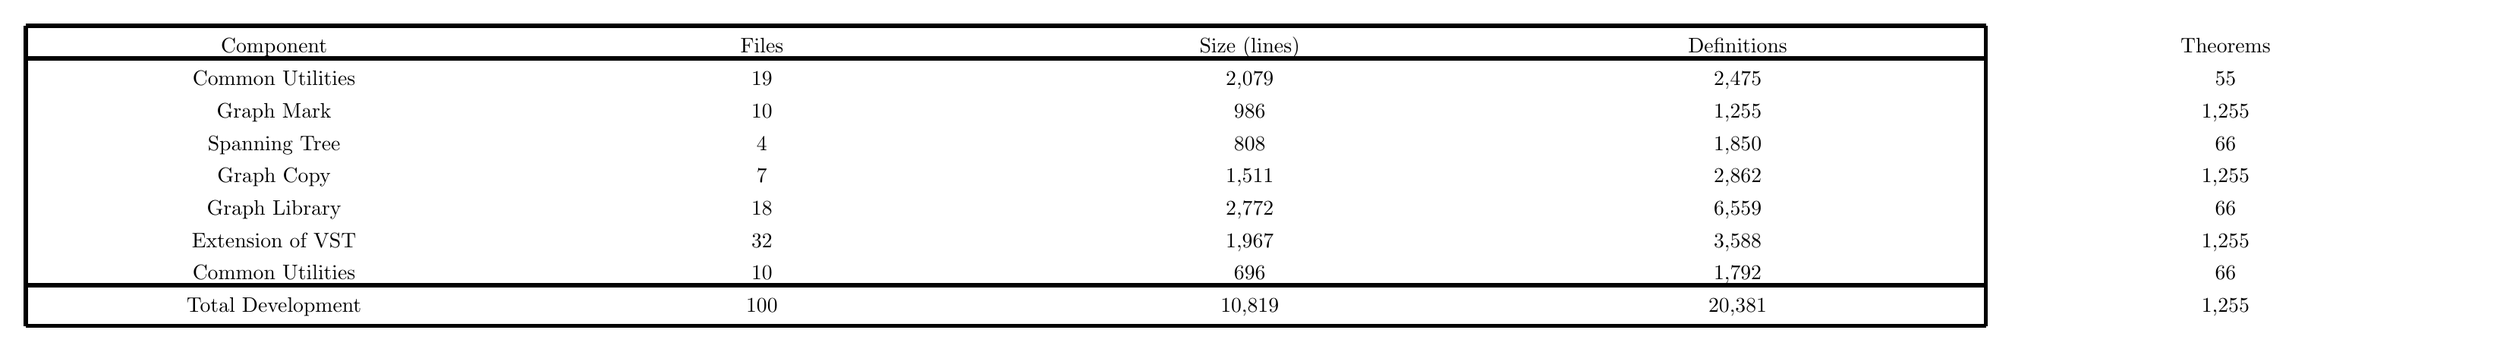
\begin{tikzpicture}[line width = 2pt]
  \matrix(stat)[
    matrix of nodes,
    ampersand replacement=\&,
    nodes={rectangle, align=center,text width=8cm},
    row sep=-\pgflinewidth,
    column sep=-\pgflinewidth,
    text depth=0.5ex,
    text height=2ex
  ]{
    |[fill=backgroundcolor]| Component \& |[fill=backgroundcolor]| Files \& |[fill=backgroundcolor]| Size (lines) \& |[fill=backgroundcolor]| Definitions \& |[fill=backgroundcolor]| Theorems \\
    Common Utilities  \& 19 \& 2,079 \& 2,475 \& 55 \\ 
    |[fill=backgroundcolor]| Graph Mark \& |[fill=backgroundcolor]| 10 \& |[fill=backgroundcolor]| 986 \& |[fill=backgroundcolor]| 1,255 \& |[fill=backgroundcolor]| 1,255 \\
    Spanning Tree  \& 4 \& 808 \& 1,850 \& 66 \\
    |[fill=backgroundcolor]| Graph Copy \& |[fill=backgroundcolor]| 7 \& |[fill=backgroundcolor]| 1,511 \& |[fill=backgroundcolor]| 2,862 \& |[fill=backgroundcolor]| 1,255\\
    Graph Library \& 18 \& 2,772 \& 6,559 \& 66\\
    |[fill=backgroundcolor]| Extension of VST  \& |[fill=backgroundcolor]| 32 \& |[fill=backgroundcolor]| 1,967 \& |[fill=backgroundcolor]| 3,588 \& |[fill=backgroundcolor]| 1,255\\
    Common Utilities \& 10 \& 696 \& 1,792 \& 66\\
    |[fill=backgroundcolor]| Total Development \& |[fill=backgroundcolor]| 100 \& |[fill=backgroundcolor]| 10,819 \& |[fill=backgroundcolor]| 20,381 \& |[fill=backgroundcolor]| 1,255\\
  };
  \draw(stat-1-1.north west)--(stat-1-4.north east);
  \draw(stat-2-1.north west)--(stat-2-4.north east);
  \draw(stat-9-1.north west)--(stat-9-4.north east);
  \draw(stat-9-1.south west)--(stat-9-4.south east);
  \draw(stat-1-1.north west)--(stat-9-1.south west);
  \draw(stat-1-4.north east)--(stat-9-4.south east);
\end{tikzpicture}
}}
\end{columns}
\end{document}
